\section{Experimental Results}\label{sec:results}

\mypar{Experimental setup} The improvements were evaluated on two different platforms:
\begin{itemize}
\item Intel\textsuperscript{\textregistered} Xeon CPU E3-1220L V2 @ 2.30 GHz, gcc (Debian 4.9.2-10) 4.9.2
\item Intel\textsuperscript{\textregistered} Core i5-2500 @ 3.3 GHz, Windows 8.1 using cygwin64 with gcc 4.9.2
\end{itemize}

The program versions were compiled with the following flags: 
-std=c++11 -Wno-deprecated -Wall -W -Wextra -fPIC -march=native -O3 -DNDEBUG -fPIC
\\
For performance analysis Intel\textsuperscript{\textregistered} VTune Amplifier XE 2015 (build 403110) was used. Cycle counts were compared with the readings obtained by using the RDTSC instruction to check the accuracy of VTune Amplifier XE 2015. Measurements deviated by less than 1\%.

\mypar{Baseline}
The analysis of the baseline implementation showed a lot of potential for optimization. Most notably by reducing memory overhead caused by object creation and deletion, random reads from lookup tables and vector operations. This can also be seen in the roofline analysis \cite{Ofenbeck:14} (see figure~\ref{roofline-mixed}).

\mypar{Impact of Optimizations}
As can be seen in figure~\ref{runtime}, the overall runtime was reduced by a factor of 7 to 25 depending on input size. Most of these improvements were achieved by reducing the number of operations by a factor of 6. One particular optimization (build 6 in figure~\ref{runtime}) replaced many multiplications with one division. Due to such optimizations the performance (TODO: Performance? Should we use computational intensity instead?) of the optimized version did not improve, as indicated by the roofline analysis in figure~\ref{roofline-mixed}. Furthermore by reducing the op count and introducing divisions the division unit is now a bottle neck. (TODO: became a bottle neck, don't change the time in which you write, everything already happened)

\mypar{Memory Accesses}
Despite all the optimizations some operations (e.g. retrieving the greatest residual to determine which message to process next or graph lookup operations) are inherently non linear in memory (TODO: What do you mean with non linear? Memory intensive?). This is especially an issue if the factor graph is larger than 1 MB as then the TLB (in the systems we measured with) can no longer serve all address translations for the graph accesses. (TODO: Is this the case, how big is our graph? Theoretical versus experimental?)

\begin{figure}\centering
    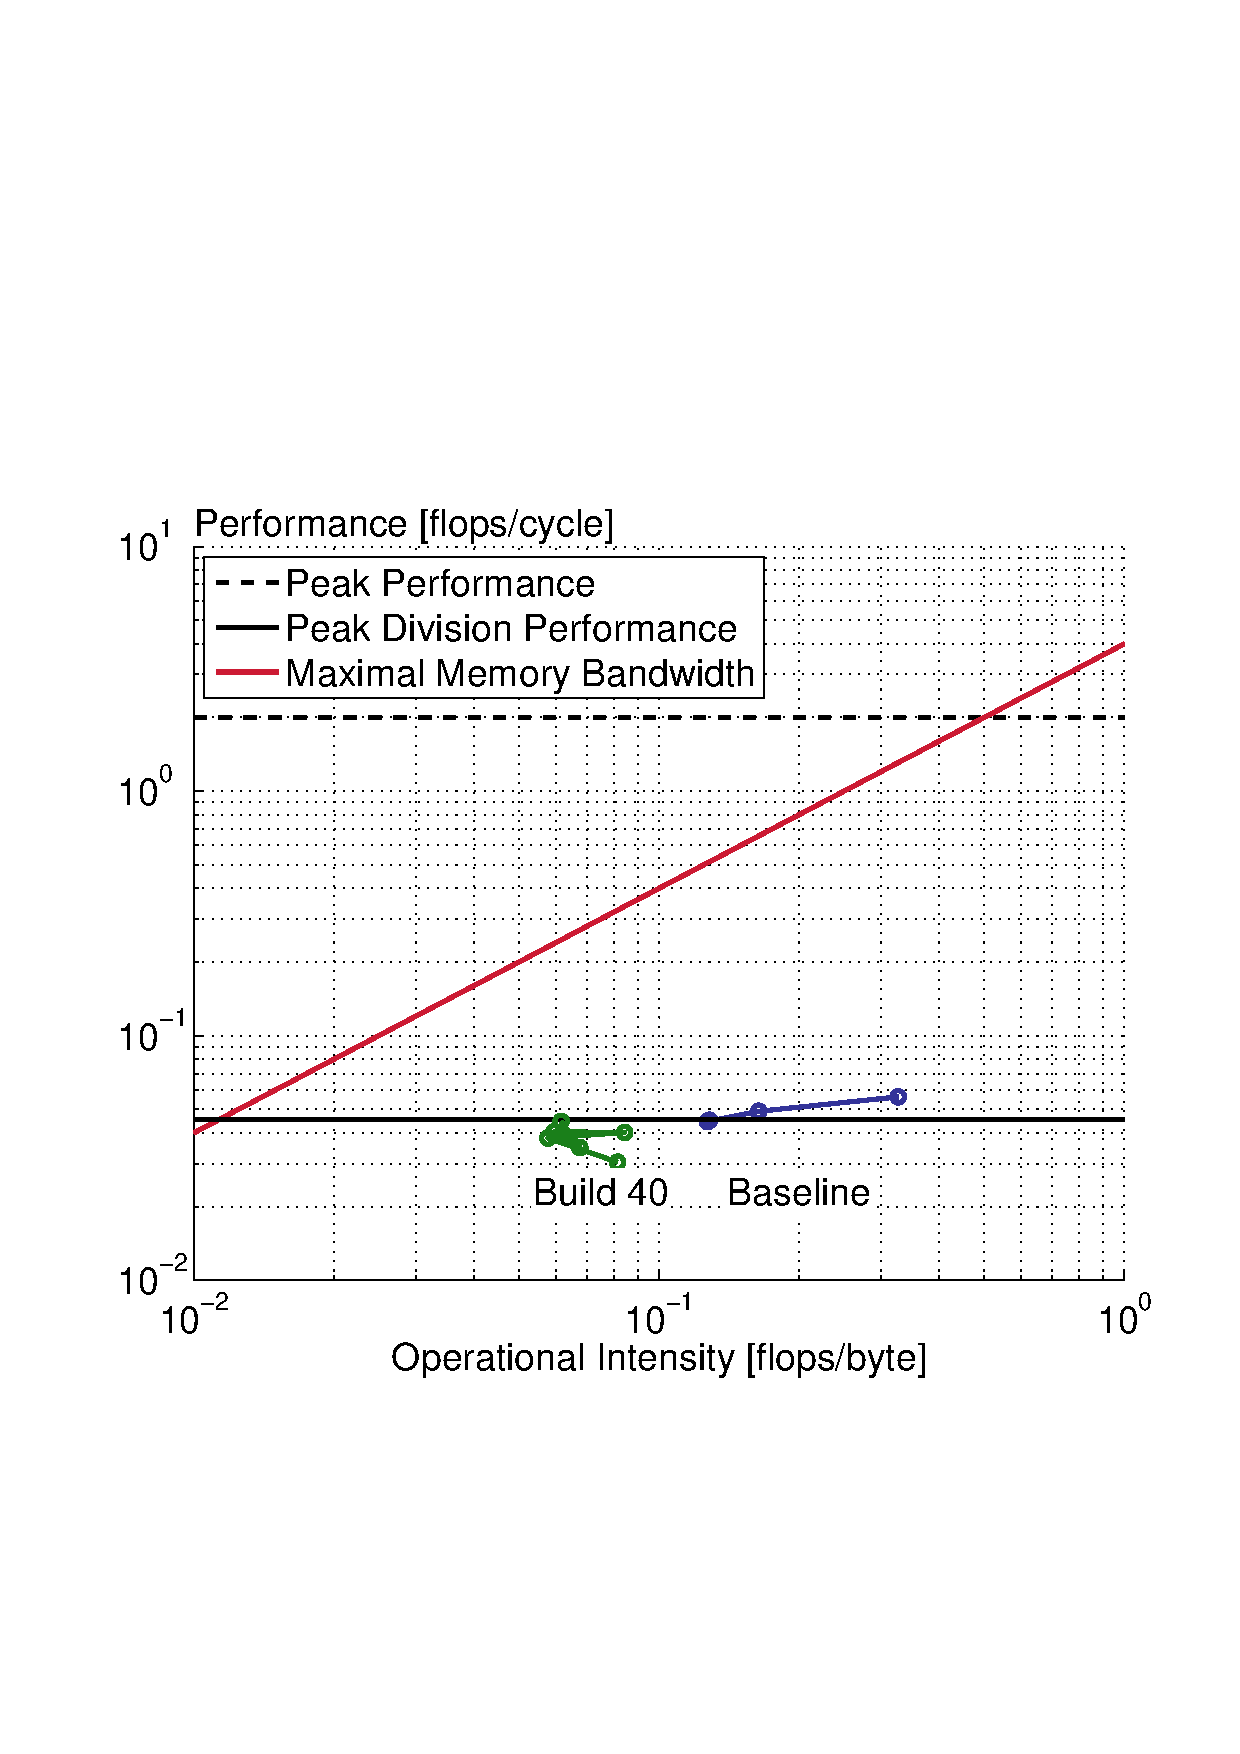
\includegraphics[scale=0.48, trim={2cm 6.5cm 1cm 8.5cm},clip]{graphics/roofline_mixed.pdf}
  \caption{Roofline analysis of the baseline and our optimized version (build 40). The analysis was conducted on the Windows system described above.\label{roofline-mixed}}
\end{figure}

\begin{figure*}\centering
  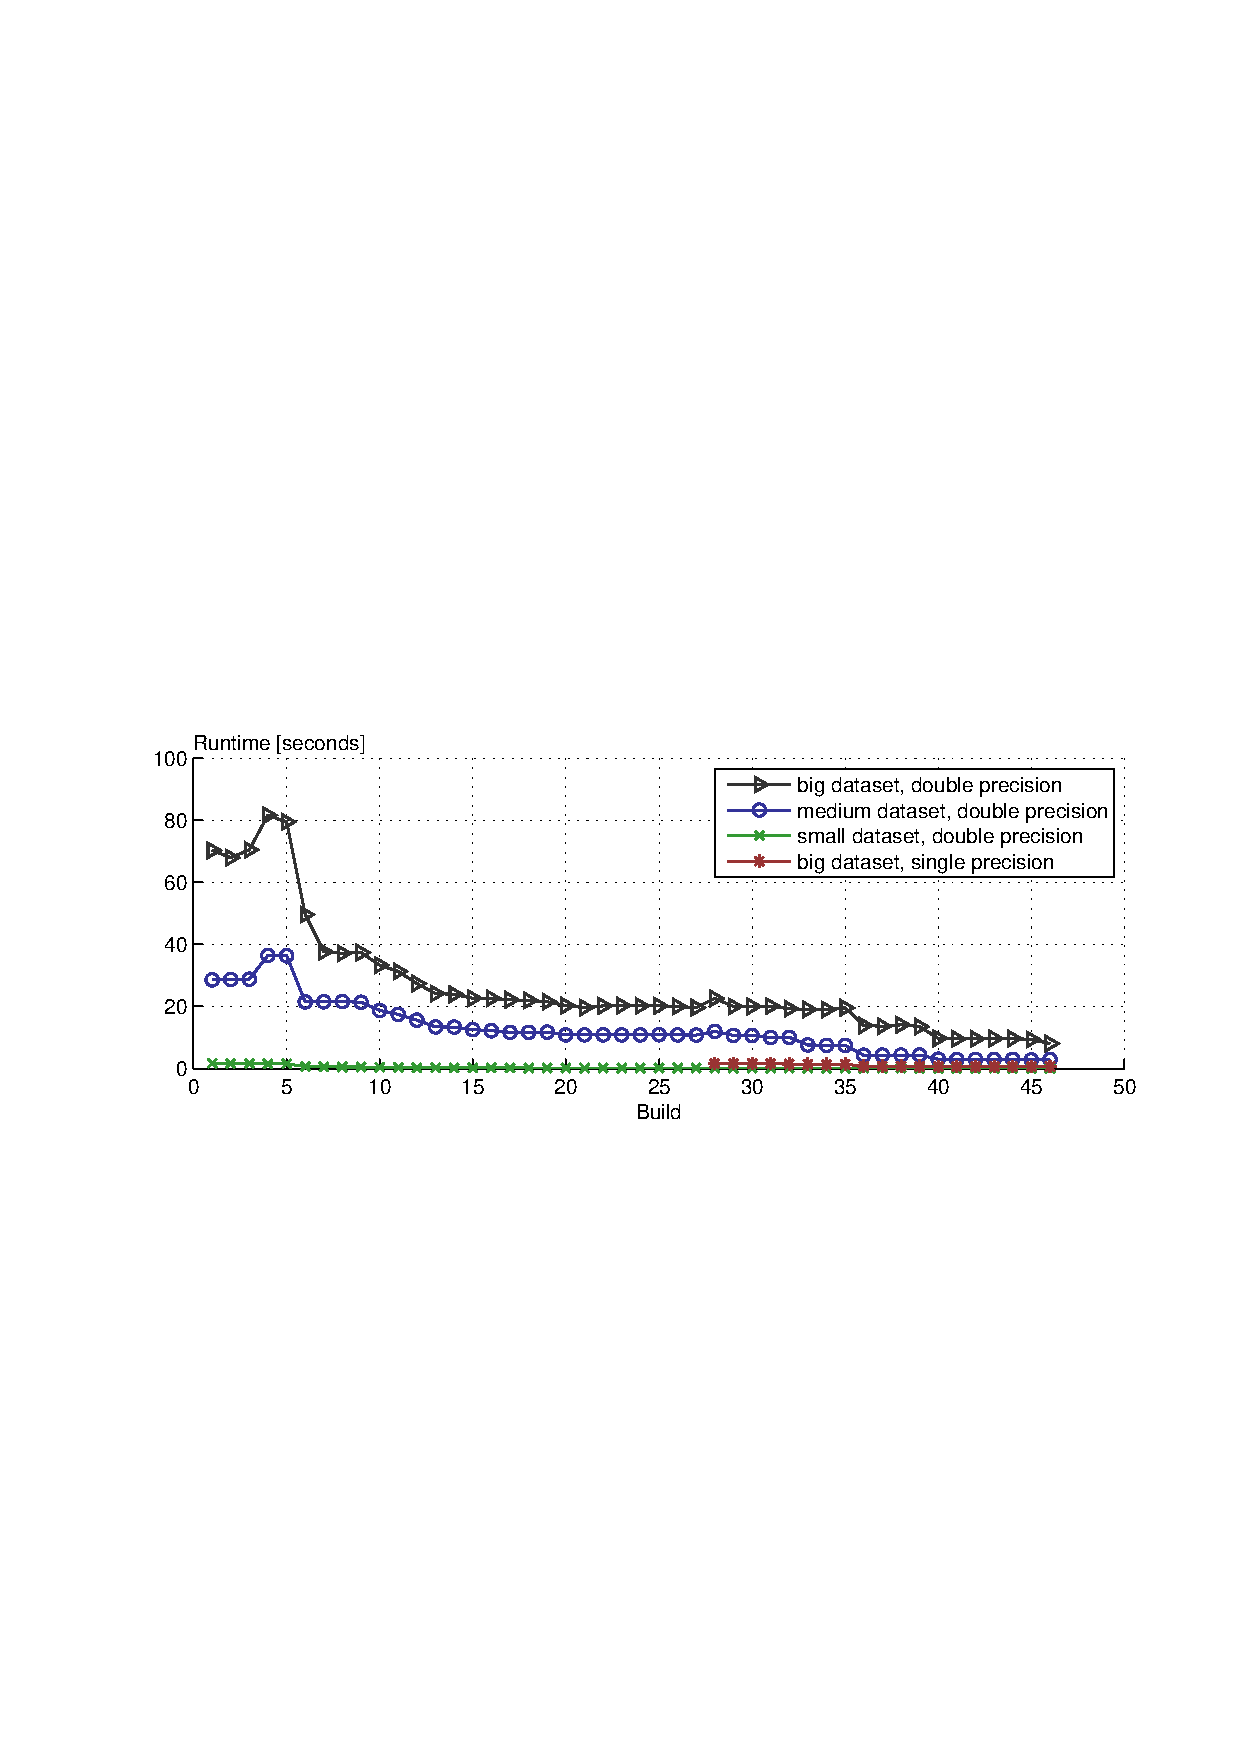
\includegraphics[scale = 1, trim={7cm 11cm 6cm 14cm}]{graphics/runtime_plot.pdf}
  \caption{Runtime plot showing the execution time on the Linux system across different versions of our program for three different input sizes.\label{runtime}}
\end{figure*}

\mypar{Vectorization}
To further improve the runtime some parts of the code were vectorized manually. Unfortunately, this did not bring a significant improvement, due to some difficulties:
\begin{itemize}
	\item The op count was reduced significantly by replacing floating point multiplications with floating point divisions (by reusing previously calculated products). This lead to a performance bound by the division unit.
	\item Vectorizing this division is not possible as the program flow depends on the result immediately, thus calculation 4 divisions at once is impossible. And calculating only one division using AVX is slower than a scalar division \cite{intrinsics_guide}. (ToDo: Explain it better, why can't we wait and do 4 at once? - Because we update single messages at random locations but need the previous residual to select the new location)
	\item Doing a scalar division results in a dependency on the write back of the floating point vector, which is expensive.
\end{itemize}
(ToDo, we tried to pre calculate the 1/x values, no use! Also special intrinsic for 1/x could not be used because accuracy was not high enough)
